\documentclass[a4paper,12pt]{extarticle}
\usepackage[table,xcdraw]{xcolor}
\usepackage{pgfplots}
\usepackage[unicode, pdftex]{hyperref}
\usepackage[T2A]{fontenc}
\usepackage[utf8]{inputenc}
\usepackage[english,russian]{babel}
\usepackage{amsmath,amsfonts,amsthm, mathtools}
\usepackage{amssymb}
\usepackage{dsfont}
\usepackage{graphicx}
\graphicspath{{images/}}
\usepackage{wrapfig}
\usepackage{floatrow}
\usepackage{setspace}
\usepackage[headings]{fancyhdr}
\usepackage[margin=10pt,font={small,stretch=0,9},labelfont=bf,labelsep=period,
justification=centerlast]{caption}
\usepackage{array,tabularx,tabulary,booktabs}
\RequirePackage{multirow}
\RequirePackage{multicol}
\RequirePackage{longtable}
\usepackage{indentfirst}
\usepackage{hyperref}
\usepackage{icomma}
\newcommand*{\hm}[1]{#1\nobreak\discretionary{}
	{\hbox{$\mathsurround=0pt #1$}}{}}
\usepackage{soulutf8} 
\usepackage{etoolbox} 
\usepackage{geometry}
\geometry{top=20mm}
\geometry{bottom=20mm}
\geometry{left=20mm}
\geometry{right=20mm}
\DeclareMathOperator{\sgn}{\mathop{sgn}}
\usepackage[OT1]{fontenc}
\usepackage{amsmath}
\usepackage{amsfonts}
\usepackage{amssymb}
\usepackage{wasysym}
\usepackage{wrapfig}
\usepackage{physics}
\usepackage[normalem]{ulem}
\graphicspath{{pictures/}}
\DeclareGraphicsExtensions{.png,.jpg,.jpeg}
\usepackage{indentfirst}
\usepackage[T2A]{fontenc}
\usepackage{subfigure}
\usepackage{fancyhdr}
\usepackage{caption}

\usepackage{tabularx}
\usepackage{floatrow}
\usepackage{multicol}
\usepackage{lastpage}

\pgfplotsset{
  MyStyle1/.style={
    axis lines = middle,
    enlargelimits = true,
    grid=both,
    grid style={line width=.1pt, draw=gray!10},
    major grid style={line width=.2pt,draw=gray!50},
    minor tick num=5,
    enlargelimits=0.05,
    ticklabel style={font=\tiny,fill=white},
    xlabel style={at={(ticklabel* cs:1)},anchor=north west},
    ylabel style={at={(ticklabel* cs:1)},anchor=south east},
  }
}
\def\Slope{1.5}
\def\Intercept{-20}


% Настройка отчёркиваний и нумерации
\usepackage{fancyhdr}
\pagestyle{fancy}
\fancyhf{}

\fancyhead[L]{\nouppercase{\leftmark\hfill}}
\fancyfoot[RO, RE]{Страница \thepage \ из \pageref{LastPage}}
\renewcommand{\headrulewidth}{0.5pt}
\renewcommand{\footrulewidth}{0.5pt}

\usepackage{titlesec}
\titlelabel{\thetitle.\quad}

\pgfplotsset{compat=1.18}
\begin{document}

\thispagestyle{empty}
\begin{center}
	\textit{Федеральное государственное автономное образовательное\\ учреждение высшего образования }
	
	\vspace{0.5ex}
	
	\textbf{«Московский физико-технический институт\\ (национальный исследовательский университет)»}
\end{center}

\vspace{10ex}
\begin{figure}[!h]
  \begin{center}
    
\includegraphics[width = 0.8\textwidth]{MIPT.png}
  \end{center}
\end{figure}

\begin{center}
	
	\textbf{Лабораторная работа №5.1.1}
	
	\vspace{1ex}
	
	по курсу общей физики
	
	на тему:
	
	\textbf{\textit{<<Фотоэффект>>}}
	
	\vspace{20ex}
	
	\begin{flushright}
		\noindent
		\textit{Работу выполнили:}\\  
		\textit{Галимов Данил \\ Легких Никита \\(группа Б05-301)}
	\end{flushright}
	\vfill
	Долгопрудный \\ \today
	\setcounter{page}{1}
\end{center}
\newpage

% Конец шаблона
\newpage

\newpage
\section*{Введение}
\textbf{Цель работы:} Исследовать зависимость фототока от величины задерживающего потенциала и частоты падающего излучения, вычислить величину постоянной Планка.

    \section*{Теоретическая часть}

    Фотоэффект --- явление испускания электронов фотокатодом, облучаемым светом,  Это явление хорошо объясняется фотонной теорией света. Взаимодействие монохроматического света с веществом можно описывать
	как взаимодействие с веществом частиц, называемых фотонами, которые обладают энергией $ \hbar \omega $ и импульсом $ \hbar\omega/c $. При столкновении фотона с электроном фотокатода энергия отона полностью передается электрону, и фотон прекращает свое существование. Энергетический баланс этого взаимодействия для вылетающих электронов
	описывается уравнением
	
	\begin{equation}\label{energy balance}
	\hbar \omega = E_{max} + W
	\end{equation}
	
	\begin{wrapfigure}{l}{0.4\linewidth}
		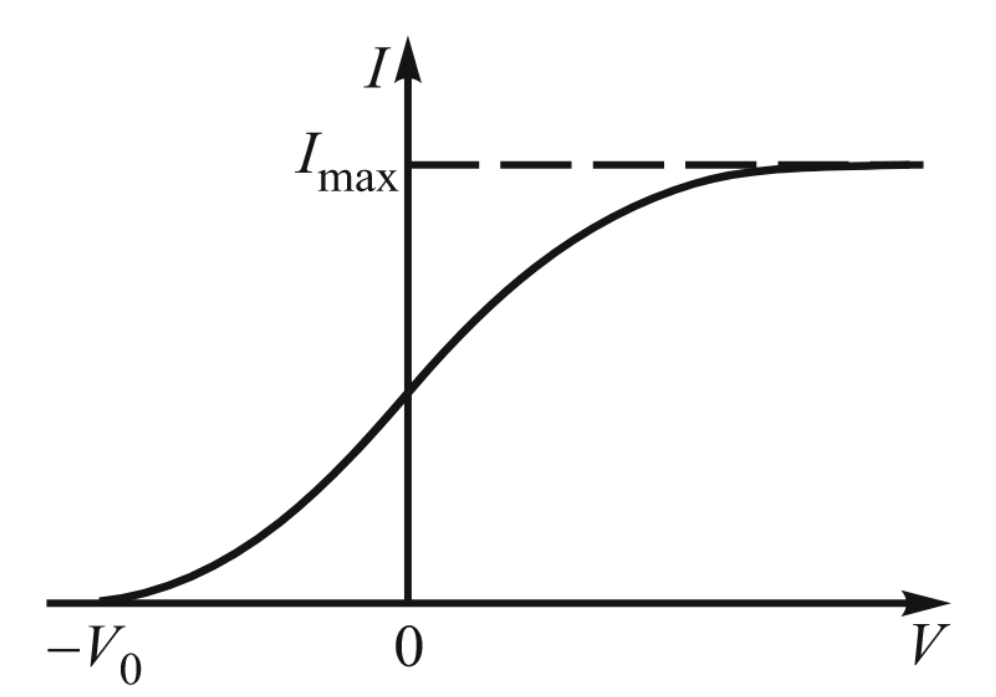
\includegraphics[width=\linewidth]{pics/I_V.png}
		\caption{Зависимость фототока от напряжения на аноде фотоэлемента}
		\label{ris I(V)}
	\end{wrapfigure}
	
	Здесь $ E_{max} $ ---  максимальная кинетическая энергия электрона после выхода из фотокатода, $ W $ --- работа выхода электрона из катода. Реально энергетический спектр вылетевших из фотокатода электронов непрерывен --- он простирается от нуля до $ E_{max} $. 
	
	Для измерения энергии вылетевших фотоэлектронов вблизи фотокатода
	обычно располагается второй электрод
	(анод), на который подается задерживающий ($ V < 0 $) или ускоряющий ($ V >
	0 $) потенциал. При достаточно больших
	ускоряющих напряжениях фототок достигает насыщения (рис. \ref{ris I(V)}): все испущенные электроны попадают на анод.
	
	При задерживающих потенциалах на анод попадают лишь электроны,
	обладающие достаточно большой кинетической энергией, в то время
	как медленно движущиеся электроны заворачиваются полем и возвращаются на катод. При некотором значении $ V = -V_0 $ (потенциал запирания) даже наиболее быстрые фотоэлектроны не могут достичь
	анода.
	Максимальная кинетическая энергия $ E_{max} $ электронов связана с
	запирающим потенциалом $ V_0 $ очевидным соотношением $ E_{max} = eV_0 $. Тогда \eqref{energy balance} примет вид, называемый уравнением Эйнштейна:
	
	\begin{equation}\label{Einsteain}
	eV_0 = \hbar\omega - W 
	\end{equation}
	
	Чтобы определить величину запирающего
	напряжения, нам надо правильно экстраполировать получаемую токовую зависимость к нулю, т. е. определить, какова функциональная
	зависимость $ I(V) $. Расчет для простейшей геометрии --- плоский катод, освещаемый светом, и параллельный ему анод --- приводит к зависимости
	
	\begin{equation}\label{sqrt I = V}
	\sqrt{I} \propto V_0 - V
	\end{equation}
	
	т. е. корень квадратный из фототока линейно
	зависит от запирающего напряжения. Эта зависимость хорошо описывает экспериментальные данные.
	
	В работе изучается зависимость фототока из фотоэлемента от величины задерживающего потенциала $ V $ для различных частот света $ \omega $, лежащих в видимой области спектра. С целью экспериментальной
	проверки уравнения Эйнштейна определяются потенциалы запирания
	$ V_0 $ при разных частотах света и строится зависимость $ V_0(\omega) $, которая, как это следует из \eqref{Einsteain}, должна иметь вид
	
	\begin{equation}\label{V(w)}
	V_0 (\omega) = \dfrac{\hbar\omega - W}{e}
	\end{equation}
	
		\begin{wrapfigure}{r}{0.4\linewidth}
		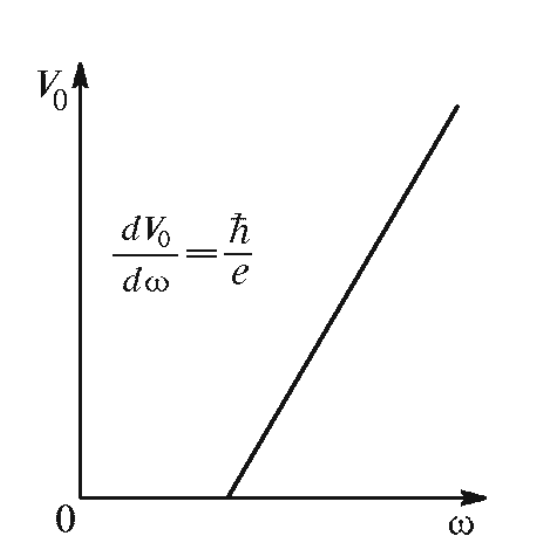
\includegraphics[width=\linewidth]{pics/V_w.png}
		\caption{Зависимость запирающего потенциала
			от частоты света}
		\label{ris V(w)}
	\end{wrapfigure}
	
	Потенциал запирания $ V_0 $ для любого катода линейно зависит от
	частоты света $ \omega $. По наклону прямой на графике $ V_0(\omega) $ (рис. \ref{ris V(w)}) можно определить постоянную Планка:
	
	\begin{equation}\label{dV/dw}
	\dfrac{dV_0}{d\omega} = \dfrac{\hbar}{e}
	\end{equation}
	
	Как показывает формула \eqref{dV/dw}, угол наклона прямой $ V_0(\omega) $ не зависит от рода вещества, из которого изготовлен фотокатод. От рода вещества, однако, зависит величина фототока, работа выхода $ W $ и форма кривой $ I(V) $ (рис. \ref{ris I(V)}). Все это определяет выбор пригодных для
	опыта катодов.

\section*{Экспериментальная установка}
Схема установки приведена на рисунке 1. Свет от источника $S$ с помощью конденсора фокусируется на входную щель призменного монохроматора УМ-2, выделяющего узкий спектральный интервал, и попадает на катод фотоэлемента Ф-25. Основные элементы монохроматора представлены на рисунке 2.
\begin{figure}[H]
  \centering
  \begin{minipage}[b]{0.45\textwidth}
    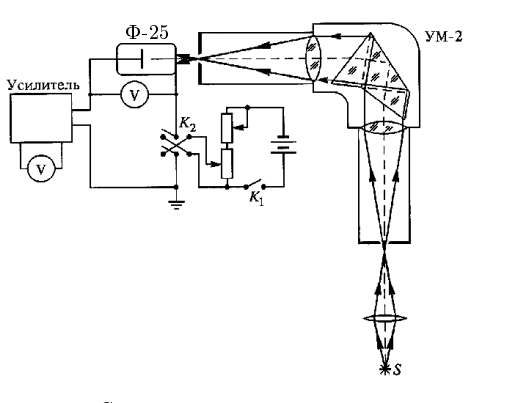
\includegraphics[width=\textwidth]{pics/scheme1.png}
  \end{minipage}
  \hfill
  \begin{minipage}[b]{0.45\textwidth}
    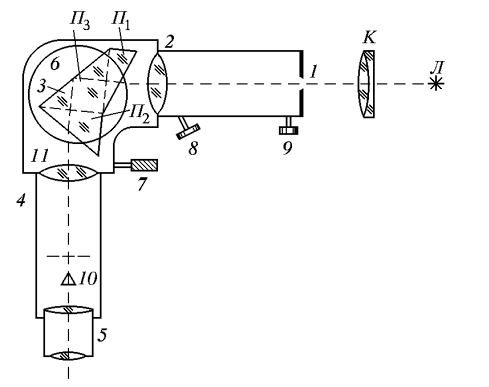
\includegraphics[width=\textwidth]{pics/scheme2.png}
    \caption{Схема экспериментальной установки}
  \end{minipage}
\end{figure}
В работе используются цифровые мультиметры модели GW Instek GDM-8145, погрешности для показаний которых считаются так в используемых нами диапазонах:
\begin{enumerate}
    \item 20V: $\sigma_V = \pm \left( 0.001 \cdot |V| + 0.05 \right)$
    \item 2V: $\sigma_V = \pm \left( 0.001 \cdot |V| + 0.005 \right)$
\end{enumerate}

\section*{Ход работы}
\subsection*{Градуировка монохроматора}
Пользуясь таблицей из справочных материалов, проградуируем барабан монохроматора по спектру неоновой лампы. Полученные результаты внесем в таблицу ниже:
\begin{table}[H]
    \centering
    \begin{tabular}{|c|c|c|c|c|c|}
    \hline
    $\lambda$, \AA & 5331 & 5341 & 5401 & 5852 & 5882 \\
    \hline
    $\varphi$, $^{\circ}$ & 2205 & 2212 & 2254 & 2513 & 2529 \\
    \hline
    $\lambda$, \AA & 5945 & 5976 & 6030 & 6074 & 6096 \\
    \hline
    $\varphi$, $^{\circ}$ & 2560 & 2574 & 2600 & 2618 & 2628 \\
    \hline
    $\lambda$, \AA & 6143 & 6164 & 6217 & 6267 & 6305 \\
    \hline
    $\varphi$, $^{\circ}$ & 2649 & 2658 & 2682 & 2702 & 2719 \\
    \hline
    $\lambda$, \AA & 6334 & 6383 & 6402 & 6507 & 6533 \\
    \hline
    $\varphi$, $^{\circ}$ & 2731 & 2750 & 2759 & 2798 & 2806 \\
    \hline
    $\lambda$, \AA & 6599 & 6678 & 6717 & 6929 & 7032 \\
    \hline
    $\varphi$, $^{\circ}$ & 2833 & 2860 & 2873 & 2944 & 2972 \\
    \hline
    \end{tabular}
    \caption{Градуировка монохроматора}
\end{table}
Погрешность измерений угла поворота монохроматора будем считать равной половине цены деления, то есть $\sigma_{\varphi} = 1^{\circ}$.\\
На основании полученных данных построим график соответствующей зависимости

\begin{minipage}{1\textwidth}
      \begin{tikzpicture}
        \begin{axis}[
          width=0.9\textwidth,
          height=,
          xlabel={$\varphi,^\circ$},
          ylabel={$\lambda$, \AA},
          MyStyle1,
          ]
          \draw[blue, domain=0:4000] plot (\x,0.0011588149359074151*\x*\x - 3.810280866205571*\x + 8102.003149362274);
          \addplot[purple, only marks] plot table [
                      x=phi, y=lambda, col sep=comma] {tables/calibration.csv};
        \end{axis}
      \end{tikzpicture}
    \end{minipage}
    
В силу нелинейности зависимости проведем квадратичную аппроксимацию.
\subsection*{Исследование зависимости фототока от величины запирающего потенциала}
Теперь проведем измерений зависимости фототока от напряжения для разных длин волн падающего света, изменяя на монохроматоре параметр $\varphi$ и переводя его в длину волны с помощью градуировки. В силу устройства установки вместо тока будем измерять пропорциональное ему напряжение $V_{I}$.\\
Для первой выбранной длины волны ($ \varphi = 2560^\circ, \lambda = (5944 \pm 2) \mathring{A}$) проведем измерения во всем спектре возможных напряжений. Результаты внесем в таблицу ниже:
\begin{table}[H]
    \begin{center}
        \begin{tabular}{|c|c|c|c|c|c|c|}
            \hline
            № & $V$, В & $\sigma_V$, В & $V_I$, В & $\sigma_{V_I}$, В & $ \sqrt{V_I}$, $\text{В}^{1/2}$ & $\sigma_{\sqrt{V_I}}$, $\text{В}^{1/2}$ \\
            \hline
            1.  & 6.71  & 0.06  & 0.581 & 0.006 & 0.762 & 0.003 \\
            2.  & 6.33  & 0.06  & 0.579 & 0.006 & 0.761 & 0.003 \\
            3.  & 5.79  & 0.06  & 0.575 & 0.006 & 0.758 & 0.003 \\
            4.  & 5.24  & 0.06  & 0.569 & 0.006 & 0.754 & 0.003 \\
            5.  & 4.65  & 0.05  & 0.561 & 0.006 & 0.749 & 0.003 \\
            6.  & 4.19  & 0.05  & 0.553 & 0.006 & 0.744 & 0.003 \\
            7.  & 3.59  & 0.05  & 0.542 & 0.006 & 0.736 & 0.003 \\
            8.  & 3.11  & 0.05  & 0.535 & 0.006 & 0.731 & 0.003 \\
            9.  & 2.53  & 0.05  & 0.511 & 0.006 & 0.715 & 0.003 \\
            10. & 2.09  & 0.05  & 0.487 & 0.005 & 0.698 & 0.004 \\
            11. & 1.45  & 0.05  & 0.430 & 0.005 & 0.656 & 0.004 \\
            12. & 0.92  & 0.05  & 0.345 & 0.005 & 0.587 & 0.004 \\
            13. & 0.39  & 0.05  & 0.172 & 0.005 & 0.415 & 0.006 \\
            14. & 0.02  & 0.05  & 0.070 & 0.005 & 0.265 & 0.009 \\
            15. & -0.02 & 0.05  & 0.054 & 0.005 & 0.232 & 0.011 \\
            16. & -0.21 & 0.05  & 0.032 & 0.005 & 0.179 & 0.014 \\
            17. & -0.32 & 0.05  & 0.011 & 0.005 & 0.105 & 0.024 \\
            18. & -1.10 & 0.05  & -0.004 & 0.005 & -0.063 & 0.040 \\
            19. & -1.78 & 0.05  & -0.005 & 0.005 & -0.070 & 0.036 \\
            20. & -3.07 & 0.05  & -0.005 & 0.005 & -0.070 & 0.036 \\
            \hline 
        \end{tabular} 
        \caption{Результаты измерений и обработка данных для $ \varphi = 2560^\circ $}
    \end{center}
\end{table}
Построим график зависимости $\sqrt{V_I}(V)$, на нем проведем прямую, аппроксимирующую линейный участок зависимости, коэффициенты которой найдем с помощью МНК (этот и дальнейшие расчеты проведены на python с помощью соответствующих пакетов - numpy, pandas):

\begin{minipage}{1\textwidth}
      \begin{tikzpicture}
        \begin{axis}[
          width=1\textwidth,
          height=,
          xlabel={$V$, В},
          ylabel={$ \sqrt{V_I}$, $\text{В}^{1/2}$},
          MyStyle1,
          ]
          \draw[red, domain=-10:10] plot (\x,0.383*\x + 0.247);
          \addplot [only marks] plot [error bars/.cd,
                x dir=both, x explicit,
                y dir=both, y explicit,
                      ] table [
                      x=V, y=I,
                x error minus=errV, x error plus=errV, y error minus=errI, y error plus=errI, col sep=comma] {tables/sqrtV-V.csv};
        \end{axis}
      \end{tikzpicture}
    \end{minipage}

Теперь проведем еще 4 серии таких же измерений для других длин волн падающего света, но уже лишь при достаточно малых значениях тока и напряжения (т.е. вблизи потенциала запирания, где искомая зависимость описывается формулой $\sqrt{V_I} \propto (V_0 - V)$). Результаты измерений внесем в таблицу ниже:
\begin{table}[H]
	\begin{center}
		\begin{tabular}{|c|c|c|c|c|c|c|}
			\hline
			№ & $V$, В & $\sigma_V$, В & $V_I$, В & $\sigma_{V_I}$, В & $ \sqrt{V_I}$, $\text{В}^{1/2}$ & $\sigma_{\sqrt{V_I}}$, $\text{В}^{1/2}$ \\
			\hline
			\multicolumn{7}{|c|}{Для $\varphi = 2618^\circ$} \\
			\hline
			1. & 0.945 & 0.005 & 0.333 & 0.005 & 0.577 & 0.004 \\
			2. & 0.649 & 0.005 & 0.253 & 0.005 & 0.503 & 0.005 \\
			3. & 0.246 & 0.005 & 0.124 & 0.005 & 0.352 & 0.007 \\
			4. & 0.405 & 0.005 & 0.183 & 0.005 & 0.428 & 0.006 \\
			5. & 0.698 & 0.005 & 0.287 & 0.005 & 0.536 & 0.005 \\
			6. & 0.083 & 0.005 & 0.086 & 0.005 & 0.293 & 0.009 \\
			7. & 0.025 & 0.005 & 0.074 & 0.005 & 0.272 & 0.009 \\
			8. & -0.830 & 0.005 & 0.008 & 0.005 & 0.089 & 0.028 \\
			\hline 
			\multicolumn{7}{|c|}{Для $\varphi = 2798^\circ$} \\
			\hline
			1. & 0.907 & 0.005 & 0.367 & 0.005 & 0.606 & 0.004 \\
			2. & 0.658 & 0.005 & 0.287 & 0.005 & 0.536 & 0.005 \\
			3. & 0.420 & 0.005 & 0.194 & 0.005 & 0.440 & 0.006 \\
			4. & 0.247 & 0.005 & 0.135 & 0.005 & 0.367 & 0.007 \\
			5. & 0.016 & 0.005 & 0.060 & 0.005 & 0.245 & 0.010 \\
			6. & -0.367 & 0.005 & 0.007 & 0.005 & 0.084 & 0.030 \\
			\hline 
			\multicolumn{7}{|c|}{Для $\varphi = 2702^\circ$} \\
			\hline
			1. & 0.776 & 0.005 & 0.295 & 0.005 & 0.543 & 0.005 \\
			2. & 0.556 & 0.005 & 0.235 & 0.005 & 0.485 & 0.005 \\
			3. & 0.363 & 0.005 & 0.165 & 0.005 & 0.406 & 0.006 \\
			4. & 0.089 & 0.005 & 0.082 & 0.005 & 0.286 & 0.009 \\
			5. & -0.016 & 0.005 & 0.057 & 0.005 & 0.239 & 0.010 \\
			6. & -0.141 & 0.005 & 0.032 & 0.005 & 0.179 & 0.014 \\
			7. & -0.444 & 0.005 & 0.008 & 0.005 & 0.089 & 0.028 \\
			\hline 
			\multicolumn{7}{|c|}{Для $\varphi = 2254^\circ$} \\
			\hline
			1. & 1.423 & 0.006 & 0.327 & 0.005 & 0.572 & 0.004 \\
			2. & 1.075 & 0.005 & 0.258 & 0.005 & 0.508 & 0.005 \\
			3. & 0.765 & 0.005 & 0.187 & 0.005 & 0.432 & 0.006 \\
			4. & 0.416 & 0.005 & 0.122 & 0.005 & 0.349 & 0.007 \\
			5. & 0.126 & 0.005 & 0.080 & 0.005 & 0.283 & 0.009 \\
			6. & 0.006 & 0.005 & 0.045 & 0.005 & 0.212 & 0.012 \\
			7. & -0.122 & 0.005 & 0.030 & 0.005 & 0.173 & 0.014 \\
			8. & -0.748 & 0.005 & -0.011 & 0.005 & -0.105 & 0.024 \\
			\hline
		\end{tabular}
        \caption{Результаты измерений и обработка данных}
	\end{center}
\end{table}

\newpage
Аналогично, построим графики зависимости $\sqrt{V_I}(V)$ для каждой из длин волн:

  \begin{minipage}[b]{0.48\textwidth}
          \begin{tikzpicture}
        \begin{axis}[
          width=1\textwidth,
          height=,
          xlabel={$V$, В},
          ylabel={$ \sqrt{V_I}$, $\text{В}^{1/2}$},
          MyStyle1,
          legend entries = {$\lambda = 2798$ \AA}
          ]
          \draw[red, domain=-10:10] plot (\x,0.405*\x + 0.257);
          \addplot [only marks] plot [error bars/.cd,
                x dir=both, x explicit,
                y dir=both, y explicit,
                      ] table [
                      x=V, y=I,
                x error minus=errV, x error plus=errV, y error minus=errI, y error plus=errI, col sep=comma] {tables/2798.csv};
        \end{axis}
      \end{tikzpicture}
  \end{minipage}
  \hfill
  \begin{minipage}[b]{0.48\textwidth}
    \begin{tikzpicture}
        \begin{axis}[
          width=1\textwidth,
          height=,
          xlabel={$V$, В},
          ylabel={$ \sqrt{V_I}$, $\text{В}^{1/2}$},
          MyStyle1,
          legend entries = {$\lambda = 2702$ \AA}
          ]
          \draw[red, domain=-10:10] plot (\x,0.405*\x + 0.247);
          \addplot [only marks] plot [error bars/.cd,
                x dir=both, x explicit,
                y dir=both, y explicit,
                      ] table [
                      x=V, y=I,
                x error minus=errV, x error plus=errV, y error minus=errI, y error plus=errI, col sep=comma] {tables/2702.csv};
        \end{axis}
      \end{tikzpicture}
  \end{minipage}
  \hfill
  \begin{minipage}[b]{0.48\textwidth}
    \begin{tikzpicture}
        \begin{axis}[
          width=1\textwidth,
          height=,
          xlabel={$V$, В},
          ylabel={$ \sqrt{V_I}$, $\text{В}^{1/2}$},
          MyStyle1,
          legend entries = {$\lambda = 2618$ \AA}
          ]
          \draw[red, domain=-10:10] plot (\x,0.350*\x + 0.270);
          \addplot [only marks] plot [error bars/.cd,
                x dir=both, x explicit,
                y dir=both, y explicit,
                      ] table [
                      x=V, y=I,
                x error minus=errV, x error plus=errV, y error minus=errI, y error plus=errI, col sep=comma] {tables/2618.csv};
        \end{axis}
      \end{tikzpicture}
  \end{minipage}
  \hfill
  \begin{minipage}[b]{0.48\textwidth}
    \begin{tikzpicture}
        \begin{axis}[
          width=1\textwidth,
          height=,
          xlabel={$V$, В},
          ylabel={$ \sqrt{V_I}$, $\text{В}^{1/2}$},
          MyStyle1,
          legend entries = {$\lambda = 2254$ \AA}
          ]
          \draw[red, domain=-10:10] plot (\x,0.256*\x + 0.226);
          \addplot [only marks] plot [error bars/.cd,
                x dir=both, x explicit,
                y dir=both, y explicit,
                      ] table [
                      x=V, y=I,
                x error minus=errV, x error plus=errV, y error minus=errI, y error plus=errI, col sep=comma] {tables/2254.csv};
        \end{axis}
      \end{tikzpicture}
  \end{minipage}
Все полученные из графиков результаты внесём в таблицу ниже:
\begin{table}[H]
\centering
\begin{tabular}{|c|c|c|c|c|c|c|c|c|c|c|}
\hline
 № & $\lambda$, \AA & $\sigma_{\lambda}$, \AA & $\omega$, $10^{15} \cdot \text{c}^{-1}$    & $\sigma_{\omega}$, $10^{15} \cdot \text{c}^{-1}$ & $k$ & $\sigma_k$ & $b$, В     & $\sigma_b$, В & $V_0$, В & $\sigma_{V_0}$, В \\ \hline
1 & 6144  & 266   & 3,07 & 0,13  & 0,383 & 0,017 & 0,247 & 0,007 & 0,64 & 0,03  \\ \hline
2 & 6070  & 262   & 3,11 & 0,13  & 0,350 & 0,024 & 0,27  & 0,013 & 0,77 & 0,06  \\ \hline
 3 & 6514  & 282   & 2,89 & 0,13  & 0,41  & 0,04  & 0,257 & 0,022 & 0,63 & 0,08  \\ \hline
4 & 6268  & 271   & 3,01 & 0,13  & 0,405 & 0,022 & 0,247 & 0,009 & 0,61 & 0,04  \\ \hline
5 & 5402  & 234   & 3,49 & 0,15  & 0,256 & 0,010 & 0,226 & 0,008 & 0,88 & 0,05  \\ \hline
\end{tabular}
\caption{Сводная таблица результатов}
\end{table}
На основании полученных результатов, построим график зависимости $V_0 (\omega)$:

\begin{minipage}{1\textwidth}
    \centering
      \begin{tikzpicture}
        \begin{axis}[
          width=0.8\textwidth,
          height=,
          xlabel={$w\cdot 10^{15},~\text{с$^2$}$},
          ylabel={$V_0,~\text{Вs}$},
          MyStyle1,
          ]
          \draw[red, domain=0:100] plot (\x,0.467*\x-0.744);
          \addplot [only marks] plot [error bars/.cd,
                x dir=both, x explicit,
                y dir=both, y explicit,
                      ] table [
                      x=w, y=V,
                x error minus=errw, x error plus=errw, y error minus=errV, y error plus=errV, col sep=comma] {tables/V-w.csv};
        \end{axis}
      \end{tikzpicture}
\end{minipage}

Коэффициент наклона полученной наилучшей прямой: $k = (0,5 \pm 0,3) \cdot 10^{-15}$ $\text{В} \cdot \text{с}$, из чего получаем $\hbar = ke =  0,467\cdot 10^{-15} \cdot 1,602 \cdot 10^{-19} \approx (0,75 \pm 0,44) \cdot 10^{-34} \; \text{Дж} \cdot \text{с}$, что согласуется в пределах доверительного интервала с табличным значением $ \hbar = 1,054 \cdot 10^{-34} \; \text{Дж} \cdot \text{с}$.
Также оценить красную границу спектра: 
\begin{equation}
	\omega_{\text{к}} = (1,6 \pm 0,5) \cdot 10^{15} \; с^{-1} \Rightarrow \lambda_{\text{к}} = \dfrac{2\pi c}{\omega_{\text{к}}} = (11800 \pm 3600) \mathring{A}
\end{equation}
И найти работу выхода материала катода:
\begin{equation}
	W = \hbar \omega_{\text{к}} = (1,2 \pm 0,3) \; \text{эВ}
\end{equation}
\section*{Выводы}
В ходе лабораторной работы удалось:
\begin{enumerate}
    \item на практике исследовать зависимость фототока от величины задерживающего потенциала и частоты падающего излучения
    \item оценит величину постоянной Планка: $\hbar = (0,8 \pm 0,4) \cdot 10^{-34} \; \text{Дж} \cdot \text{с}$ (что равно в пределах погрешностей табличному значению $ \hbar = 1,054 \cdot 10^{-34} \; \text{Дж} \cdot \text{с}$)
    \item оценит красную границу спектра ($\lambda_{\text{к}} = (11800 \pm 3600) \mathring{A}$) и работу выхода материала катода ($W = (1,2 \pm 0,3) \; \text{эВ}$)
\end{enumerate}

\end{document}